\chapter{Introduction}

% The Universe is comprised of just a few basic building blocks: the fundamental particles.

The Standard Model (SM) of particle physics is a collection of the most accurate and self-consistent theories which describe the particles within the Universe and their interactions with each other.
For the past century, some of the most brilliant physicists have spent their entire careers to develop equations, mathematical tricks, and completely novel ideas in order to give a solid foundation to the SM.
To demonstrate the unparalleled accuracy with which the SM makes predictions, compare the experimentally measured anomalous magnetic moment of the electron
\begin{equation*}
    a_e^{\mathrm{exp}} = 0.001\ 159\ 652\ 180\ 73(28)
\end{equation*}
to the value predicted by the SM
\begin{equation*}
    a_e^{\mathrm{pred}} = 0.001\ 159\ 652\ 181\ 643(764).
\end{equation*}
An agreement to better than one in a trillion! 
Not bad coming from those who work with only paper, pencils, and time.

First, the major players that make up the SM - the fundamental particles - are introduced.
Next, an explanation is given on how the infamous Higgs boson completed the SM.
Finally, problems of the SM are described and how its claims can be tested.
% Some of the most brilliant minds in physics have worked for their entire careers to develop equations and  novel ideas solutions to problems which perplexed mankind for more than 100 years a century's worth of work to  
% an impressively accurate 
% It is currently the most accurate model of particles and their interactions with each other - and frankly - it is {\it quite} impressive!

% Allow me to paint the picture, as I see it:
% We all are included in the Song of the Universe.
% This song is called "Reality" and this tune has been playing for nearly 13.8 billion years, or so the cosmologists tell us. 
% To me, the notes and lines on this music staff resemble particle physics.
% The staff lines are like field lines which permeate the Universe.
% I imagine them like the strings on a violin.
% When a field line is plucked, you a create a note: a particle.
% If you pluck an electromagnetic field line, you get a photon.
% If you pluck an electron field line, you get an electron.
% A Higgs field line, a Higgs boson.
% Particle Physicists are curious about these notes and strings, 
% the particles and the fields and how they interact with each other.

% So, how does the song go?

\section{The Particles: The Players on the Fields}

Contrary to intuition, fundamental particles are not hard, billiard-ball-like objects as is often perceived.
Instead the SM predicts that every particle is actually an \emph{excitation} of its corresponding field.
So for example the electron is an excitation of the \emph{electron field}, $\psi_{e}(x)$, a bispinor that describes a spin-1/2 field which follows the Dirac equation: 
\begin{equation*}
    (i\hbar c \gamma^{\mu}{\partial}_{\mu} 
    - mc^{2})\psi(x) = 0.
\end{equation*}
In fact, \emph{every} electron is an excitation of this same electron field. 
An electron is identical to every other electron in every way (same mass, same charge, etc.).
Quantum Mechanics (QM) does a fine job of describing how slow-moving particles behave.
However, as soon as particles begin moving at 30.5\% of the speed of light (91.4 $91.4 E6$ m/s), then there is a 5\% difference between the particle's rest mass energy ($E = mc^2$) and its total relativistic energy ($E = \gamma mc^2$).
In other words, fast-moving particles must account for effects due to Special Relativity (SR).
The merger of QM and SR gives rise to Quantum Field Theory (QFT) - the backbone of the SM.

Figure~\ref{fig:particulartable} shows all the fundamental particles that have been discovered up to the present day.
The phrase ``fundamental particle'' just means that the particle is not composed of anything smaller than itself. 
These particles are not just diabolical creations from theorists. 
No, these particles are precisely defined, mathematical objects whose existence has been predicted by the SM and experimentally verified time and time again in the laboratory.
%%%%%%%%%%%%%%%%%%%%
\begin{figure}[pbth]
\centering
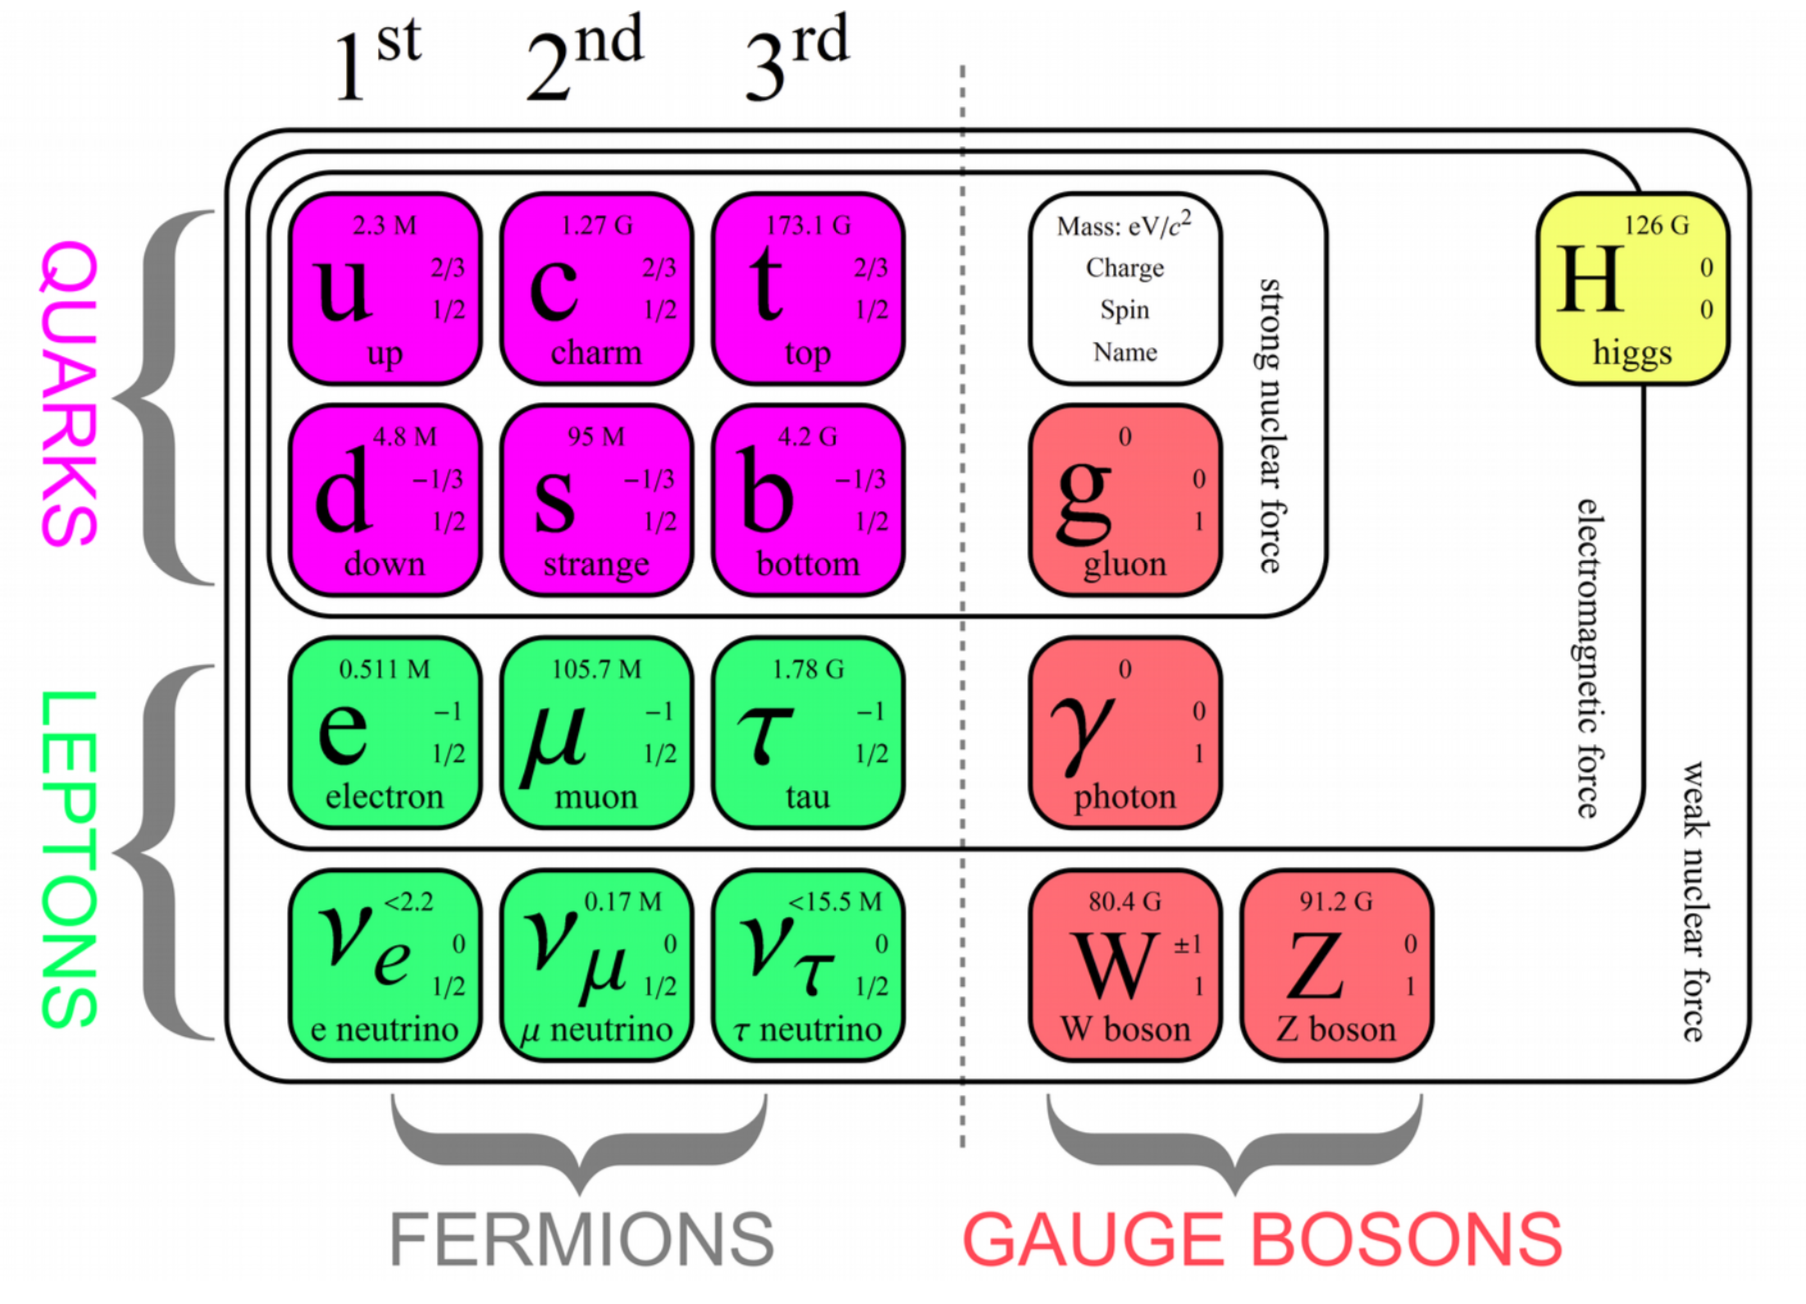
\includegraphics[width=15cm,height=15cm,keepaspectratio]{figures/sm/particular_table_updated.png}
    \caption{The fundamental particles of the Standard Model.} 
    \label{fig:particulartable}
\end{figure}
%%%%%%%%%%%%%%%%%%%%

Each particle has a unique set of properties (like mass, electric charge, spin, \etc.) that distinguish it from all the other particles. 
It is one of the primary goals of particle physics to determine these properties, because ultimately their properties determine their \emph{interactions} with one another. 

Without further ado, let's meet the particles.
There are two major types: \emph{bosons} and \emph{fermions}.
We are going to take a non-traditional route and introduce the bosons first, then the fermions.

\subsection{Bosons: Use the Force}
% The bosons are said to be the "force carrier" particles. 
% In particle physics, when two particles interact with one another, how do they do it? 
% instead an intermediate particle, very often a boson, is said to ``mediate'' the interaction and be the entity responsible which transfers the force from one particle to the other. 
Ever wonder how two electrons "know" that they are near each other and that they should repel? 
Figure~\ref{fig:ee_scattering} shows a Feynman diagram of two electrons ``communicating'' with each other by means of an intermediate photon.
I like to think of it as the two electrons ``playing catch'' with the photon.
The first electron recoils from the throw and then the second electron recoils from catching the photon.
The photon carries some momentum away from the first electron and brings it to the second one, therefore making it look as if the two electrons are repelling one another!
The photon isn't \emph{real} of course - it is said to be a \emph{virtual} photon.
Now we see why bosons are called the force carriers.
%%%%%%%%%%%%%%%%%%%%
\begin{figure}[pbth]
\centering
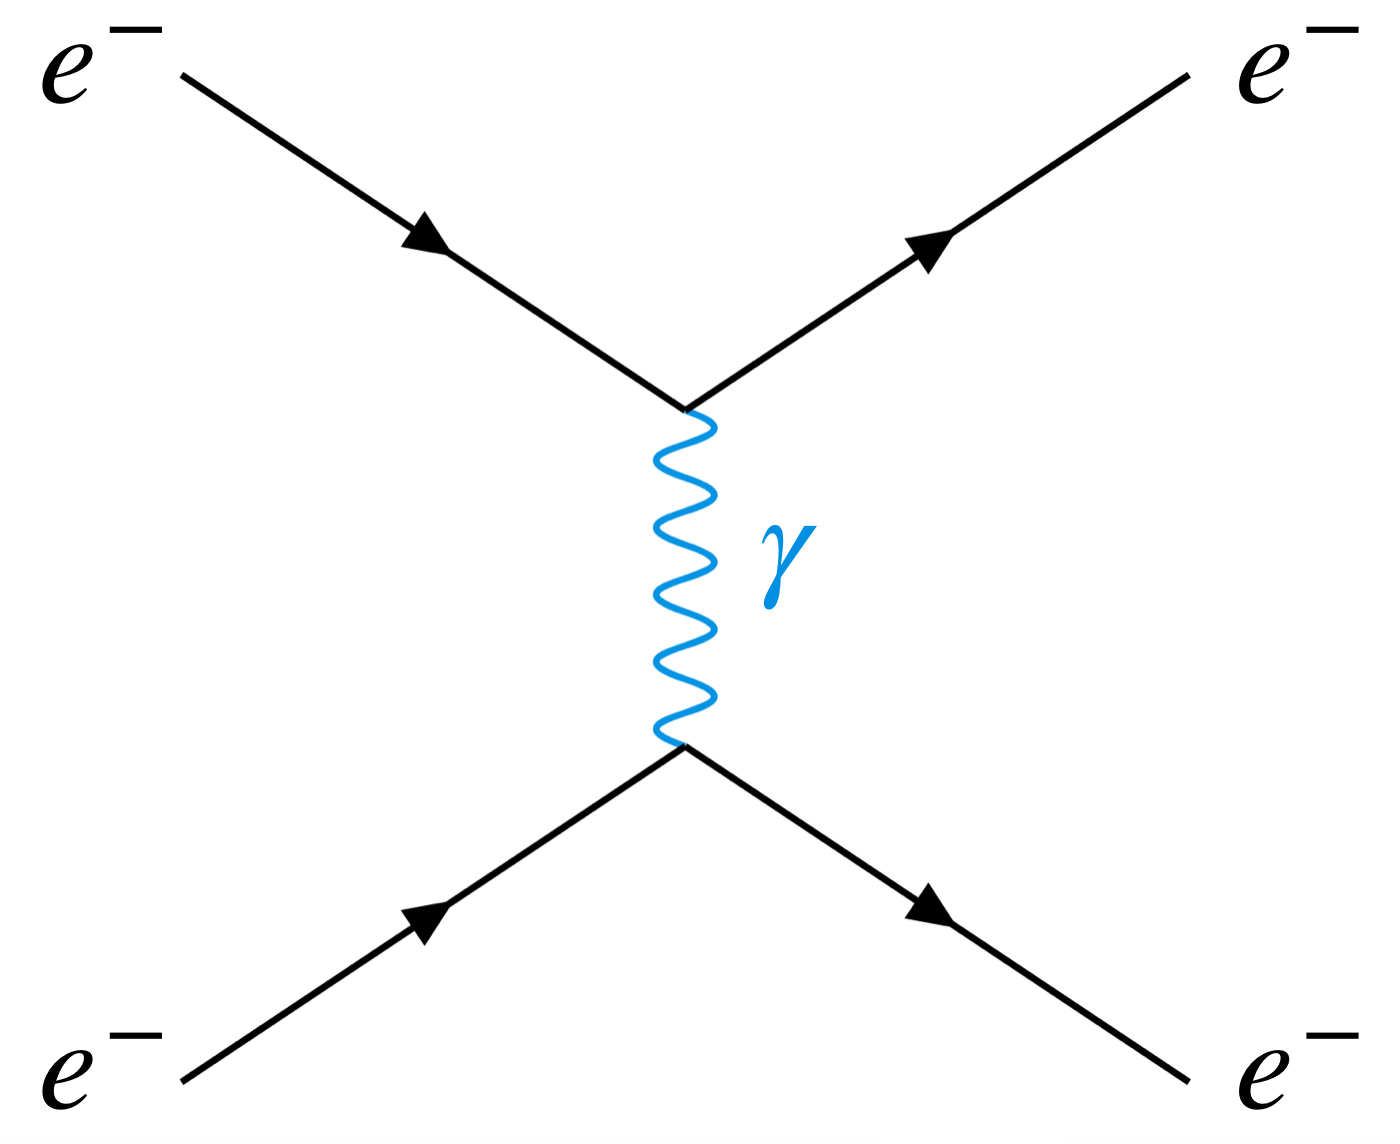
\includegraphics[width=6cm,height=6cm,keepaspectratio]{figures/sm/ee_scattering_Moeller.png}
    \caption{A Feynman diagram showing electron-electron scattering, also known as Møller scattering.} 
    \label{fig:ee_scattering}
\end{figure}
%%%%%%%%%%%%%%%%%%%%

% Quantum Electrodynamics, one of the theories cooped up in the SM, is a quantum field theory that can mathematically describe one electron "throwing" a photon to the other.
A diagram such as the one above is a Feynman diagram and it gives us a wonderfully simple way to visualize particle physics processes.
It's not \emph{actually} what happens between the particles, but it is a good starting point.
Each diagram is actually a single, scalar number -
a complicated QFT integral that tells you how likely a process is to happen.
Another benefit to Feynman Diagrams is that they are kind of like tinker toys, 
in that you can string them together in novel ways to predict real-world processes.
Quantum Electrodynamics (QED), one of the theories that make up the SM, mathematically describes and predicts the electrons mediating such a photon between them. 
It's not just limited to electrons mediating photons, however.
QED and other QFTs can predict to astounding accuracy how likely a process is to happen, between whichever particles and fields. 
You just need to know their properties first.
% \emph{Any} particle with electric charge can interact via the electromagnetic force (EM) force.

We have now met the first force carrier: the photon.
It is a massless particle and is the mediator of the EM force. 
Photons only interact with particles that carry \emph{electric charge}.
Depending on what kind of charge a particle carries, determines with which bosons it may interact and via which forces.
Speaking of forces, the four fundamental forces found in nature, along with their decreasing, relative strength are: 
% (1) strong, (2) EM, (3) weak, (4) gravitational
\begin{enumerate}
    \item strong force $(1)$
    \item EM force $(10^{-1})$
    \item weak force $(10^{-6})$
    \item gravitational force $(10^{-40})$
\end{enumerate}
If the photon is the mediator of the EM force, then what mediates the other forces?

The mediators of the strong force are the 8 {\bf gluons}. 
Similar to the photon, they are also massless, but that's about all they have in common. 
Gluons are trapped inside of protons, neutrons, and other hadronic matter. 
They are responsible for ``glueing'' nuclei to together, hence their name.
Just as photons can only interact with particles that have electric charge, gluons can only interact with particles that have \emph{color} charge.
Interestingly, gluons themselves carry color charge which they mediate back and forth between quarks (fermions discussed below).
This is quite different from the photon which itself does not carry electric charge. 
There are three kinds of color charges: red, green, and blue.
Every gluon carries two color charges:
one kind of color and an anticolor: antired, antigreen, or antiblue.

There are three bosons which mediate the weak force: the Z, W$^+$, and W$^-$.
They are extraordinarily massive particles, weighing in at 91.2 GeV for the Z and 80.4 GeV for both kinds of W bosons. 
That means the W bosons weigh more than an iron atom! These bosons interact with any particle that carries ``weak hypercharge''.
The weak force has plagued physicists for nearly a century until only recently.
Particles which decay via the weak force live an astonishingly long time. 
Take for example the neutral pion ($\pi^0$). 
It decays very quickly, via the EM force, into two photons on the order of $10^{-18}$ s.
Now take the charged Kaon ${\rm K^+}$. 
This particle decays into three charged pions, but takes on average $10^{-8}$ s to do so.
Over 10 orders of magnitude different from the pion decay.
This is because the charged kaon decays via the weak force.

The last boson not yet mentioned is the scalar Higgs boson, which is introduced in Section~\ref{sec:EWSB} below.

% 1. There are 12 kinds fermions which are the matter particles and comprise all the matter that you see and feel
% 2. And in the other group there are 5 kinds of bosons, which are the force carriers and help fermions communicate with each other. 

\subsection{Fermions: Each One Matters}
There are 12 kinds of fermions - the matter particles of the Universe. 
They comprise all the ``stuff'' that we see and feel.
All fermions have half-integer spin, typically a value of 1/2. 
The fermions can be split into two groups depending on if they interact with the strong force (quarks) or not (leptons).
Let's consider the leptons first.

{\bf Leptons:}
% Ultimately all the matter we see, feel, and interact with daily is composed of fermions.
% Referring back to Figure~\ref{fig:particulartable}, Fermions can be categorized into two groups: {\bf leptons} and {\bf quarks}.
We already introduced one lepton earlier: the electron. 
Looking again at the ``particular table'', the electron has a heavier brother, the muon, which is 200 times heavier than the electron. 
Then there is an even heavier sibling: the tauon. 
All three of these leptons have the familiar -1 charge which allows them to interact via the EM force and exchange photons with other electrically charged particles.

The charged leptons also carry weak hypercharge, which allows them to interact via the weak force. 
If a charged lepton interacts with a W$^\pm$ boson, it can transform into its corresponding ``partner'' - the other member of the $SU(2)$ isospin doublet: the neutrino.
These fickle particles are neutral and \emph{only} interact via the weak force (well, and maybe gravity). 
They are very difficult to detect.

% How do we know that some particles, like protons and neutrons are actually composed of smaller bits, like these up and down quarks?
% Through deep inelastic scattering experiments, analogous to the Rutherford experiment,
% one can shoot electrons at these nucleons and probe into them.
% Thanks to the wave-particle duality of nature, these electrons can act like little wave bullets,
% that tunnel into the nucleon and sometimes... they bounce back. 

% For each charged lepton, it can transform it into its neutral form: 
% the corresponding neutrino. 
% For example, the muon can transform into a muon neutrino - and vice versa.
% To undergo this transformation, the muon must interact 
% with the appropriate boson: W-. 
% This conserves electric charge at this vertex.

% You can also view this diagram from another perspective 
% by rotating it. 
% Here we see a 

{\bf Quarks:}
The six quarks are the fermions which interact with gluons.
They have \emph{quarky} names like: 
up, down, charm, strange, top, bottom. 
These are called the six ``flavors'' of quarks.
The top quark is an absolutely massive particle, reaching the top of the mass scale of any particle at 173 GeV - about as heavy as a tungsten atom.

Quarks are electrically charged particles, but they have fractional charge.
Each quark in the top row of Fig.~\ref{fig:particulartable} has +2/3 electric charge and the bottom row has -1/3.
That's why when you combine two up quarks with a down to form a proton quark, the combination of electric charge yields +1.

Just as the leptons carried weak hypercharge and could interact via the weak force, so too can quarks. 
The W$^{\pm}$ bosons can change one flavor of quark into another.
The Z boson only affects the spin, momentum, and energy of the particle with which it interacts.

In addition to electric charge, quarks also carry one kind of color charge, either red, green, or blue. 
It is this color charge which allows them to interact with gluons via the strong force. 
This is an artifact of being gauge bosons of the $SU(3)$ symmetry group.
They combine in different ways to form at least two types of hadrons.
The first type is baryons, like protons, neutrons, lambdas (anything that is $qqq$) and the second type is mesons, like pions, kaons, etas (anything of some form like $q\bar{q}$).
For some reason which is not completely understood, only colorless bound states form in nature. 
Just as a `$+$' charge would negate a `$-$' charge, so too would the `red' color charge negate `antired' (as in the case of an observable meson) or even combining red, green, and blue (as in the case of a baryon) would yield a colorless bound state.

{\bf Antiparticles:} It should be noted that almost every \emph{particle} has a corresponding \emph{antiparticle}, whose charges (\eg, color charge, electric charge) are all opposite the original particle's charges.
Accounting for leptons, quarks, bosons, bound states of quarks, and now antiparticles, it is easy to see why sometimes particle physics is referred to as a ``zoo''!

\section{Electroweak Symmetry Breaking and the Higgs Boson}
\label{sec:EWSB}
% At room temperature, we know that the weak force, which mediates decays of radioactive substances, is very different from the EM force.
% However, at large energy scales, like those found during the Big Bang or those produced in the energetic proton-proton collisions of the Large Hadron Collider, the electromagnetic (EM) force and weak force are unified. 
At large energy scales, like those found during the Big Bang or those produced in the energetic proton-proton collisions of the Large Hadron Collider, the electromagnetic (EM) force and weak nuclear force are one and the same: they are unified.
However, at lower temperatures (like room temperature for example), we know that the weak force is very different from the EM force.
The former mediates decays of radioactive substances, whereas the latter mediates the excitation of electrons in an atom.
So what is responsible for the separation of these two forces, this so-called \emph{electroweak symmetry breaking}?

Upon writing down the equations of motion from the SM Lagrangian (easier said than done), one discovers that all the particles mentioned earlier should have \emph{no mass}.
Well that's a problem because most particles in nature definitely have mass, like the quarks, leptons, W$^{\pm}$, and Z bosons.
% Since mass is a scalar, one can introduce a scalar field (spin 0) into the Lagrangian.
By introducing a complex SU(2) doublet of scalar fields into the SM Lagrangian, in such a way that it leaves the Lagrangian invariant, then all peace can be restored.
This scalar field turns out to be the Higgs field, and its excitations are Higgs bosons.
Doing so reveals the particle which should have mass,
The process of introducing a Higgs field and breaking the electroweak symmetry is called the {\bf Higgs Mechanism}.

% The Higgs field is required to be a scalar field and consists of a complex doublet, with four degrees of freedom.
Each particle interacts with the Higgs field with a different strength: in fact, a particle's coupling strength to the Higgs field is exactly its mass! 
The more the particle interacts with the Higgs field, the more mass it gains.
Excitations, or quanta, of the Higgs field are Higgs bosons and are a direct consequence of introducing a Higgs scalar field into the SM Lagrangian to allow particles to have mass.

\section{The Standard Model Doesn't Explain Everything}
The SM has only mathematically accommodated the strong, EM, and weak forces.
One problem however is that the SM can't predict the mass of the Higgs boson... or the mass of \emph{any} particle for that matter.
That's not the only thing the SM has trouble doing. 
For example, the SM can't...
\begin{itemize}
    \item ...incorporate gravity into its mathematical framework.
    \item ...explain why most of the Universe is made of matter and very little antimatter.
    \item ...predict the existence of dark matter - but we know it's there from observation.
    \item ...explain why there should be exactly three generations of fermions. 
\end{itemize}

So we see that the SM isn't the ultimate Theory of Everything, but it does a pretty good job. 
How can we test the SM and try to break it or confirm it?
There are at least two routes to choose from:
A patient route and an impatient route.
The patient route requires us to wait until our particles of interest
maybe come from outer space or, if we produce it in the lab, 
wait for it to decay into other particles. 
This could take a VERY long time, (possibly way longer than the age of the Universe - if a proton even decays at all!),
or it could take as short as a billionth of a billionth of a millionth of a second, 
like in the case of a ${\rm Z}$ boson.
It's not the most reliable method, it is difficult to control, and it requires a lot of patience.

Instead, let's be impatient: 
let's smash particles together and convert their energies into new kinds of matter. 
If we use hadrons, which are made of smaller parts like, quarks and gluons 
(let's call them ``partons'') then we will have many more interactions and a lot more fun (Fig.~\ref{fig:pp_collision}).
We are going to need a lot of energy, so we should make a large collider. 
Let's make a Large Hadron Collider!
%%%%%%%%%%%%%%%%%%%%
\begin{figure}[pbth]
\centering
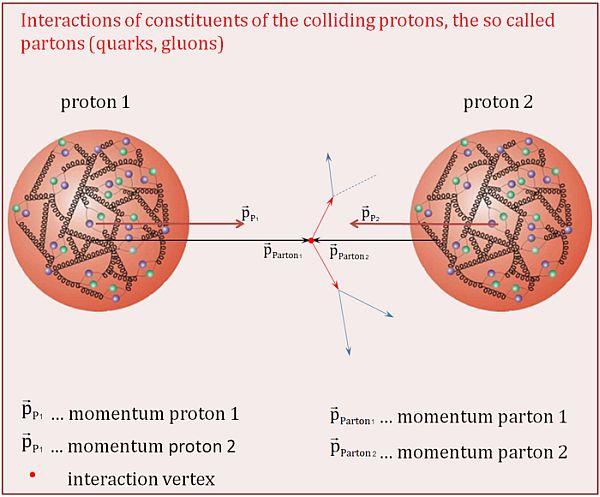
\includegraphics[width=15cm,height=15cm,keepaspectratio]{figures/lhc/proton_proton_quarksandgluons.jpg}
    \caption{
    Two protons can be smashed together at very high energies to have their partons interact and convert the high energies into new kinds of matter.} 
    \label{fig:pp_collision}
\end{figure}
%%%%%%%%%%%%%%%%%%%%